% ---------
% --------
%!TEX TS-program = pdflatex
%!TEX encoding = UTF-8 Unicode
%!TEX spellcheck = English (Aspell)

\documentclass[11pt]{article}
\usepackage{jeffe,handout,graphicx}
\usepackage{fourier-orns}
\usepackage{mathtools}
\usepackage[normalem]{ulem} % either use this (simple) or
\usepackage{tikz}
\pagestyle{empty}

\allowdisplaybreaks

\begin{document}


\begin{center}
\Large\textbf{CSCI 332, Fall 2025}%
\\
\LARGE\textbf{In-class Activity}%
\end{center}

Recall the definition of the $n$th Fibonacci number:

% cases for fibonacci numbers:
\begin{equation*}
   F(n) = \begin{cases}
      0 & \text{if } n = 0 \\
      1 & \text{if } n = 1 \\
      F(n-1) + F(n-2) & \text{if } n > 1
   \end{cases}
\end{equation*}

\begin{enumerate}
   \item Write a recursive algorithm to compute $F(n)$. Check your answer
   by implementing it in Python here: https://www.online-python.com/vpEjKaXOBt.
   (Link is also in Discord.)

       \begin{algo}
    fibo($n \in \mathbb{Z}^{\geq 0}$):\+\\
    \\
    \\
    \\
    \\
    \\
    \\
    \\
    \\
    \hspace{4in}

    \end{algo}

    \item What do you notice about the runtime of your algorithm?

    \item What is the recurrence for the runtime of your algorithm? The base
    cases are filled in for you.  Remember that the recurrence should be the sum
    of the time for the recursive calls and the time for the non-recursive work.

    $T(0) = 1$, $T(1) = 1$, $T(n) = \underline{\hspace{5cm}}$ for $n > 1$.


   \item Draw the recursion tree for fibo(7). Label each node with the function call
   that is being made. The first node is filled in for you.

   \begin{center}
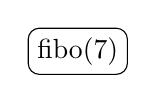
\begin{tikzpicture}
  \node[rectangle, draw, rounded corners] {fibo(7)};
\end{tikzpicture}
\end{center}

\newpage

\item What is your guess for the asymptotic number of nodes in the tree,
in terms of the input number $n$?

num. nodes is $\Theta(\underline{\hspace{3cm}})$

\item Do you see any way to improve the runtime of the algorithm?

\end{enumerate}




%%%%%%%%%%%%%%%%%%%%
\end{document}
